\chapter{Spektrometri Massa dan Spektroskopi Atom}\label{ch:b2:mass-spec-atomic}

Kembang api berwarna merah karena garam stronsium, hijau karena garam
barium, kuning karena natrium: nyala api mengubah atom menjadi cahaya
dengan warna-warna yang mengenalinya. Spektrometer massa, yang
penampilannya lebih bersahaja, menimbang molekul-molekul tunggal,
memilahnya menurut isotopnya, dan memecahnya menjadi potongan-potongan yang
massanya menunjukkan bagaimana molekul itu dibangun. Kedua teknik itu
menjawab pertanyaan ``apa yang ada dalam sampel ini, dan berapa banyak?''
dari jumlah yang sangat kecil, yang pertama untuk molekul, yang kedua untuk
unsur.

\begin{omfigure}

\includegraphics[width=0.58\linewidth]{images/book3/ai/b2-32-fireworks.jpg}

{\small Kembang api di atas sungai (ilustrasi). Kuning natrium adalah cahaya
atom-atomnya; merah tua dan hijau sebagian besar berasal dari
molekul-molekul kecil stronsium dan barium yang terbentuk dalam nyala.}
\end{omfigure}

\begin{recall}
Jilid sekolah: isotop dan kelimpahannya. Jilid Tahun 1: tingkat energi dan
garis spektrum, absorbans dan hukum Beer--Lambert, karbokation dan radikal,
derajat ketidakjenuhan. \Cref{ch:b2:chromatography}: \omterm{def:b2:chromatography:techniques}{kromatografi gas}, yang
sering mengumpani spektrometer massa.
\end{recall}

\section{Spektrometer massa}

\begin{definition}[Spektrometri massa]\label{def:b2:mass-spec-atomic:spectrum}
Yang disebut \emph{spektrometri massa}\index{spektrometri massa} mengubah
molekul-molekul sampel menjadi ion-ion gas, memisahkan ion-ion itu menurut
\emph{rasio massa terhadap muatan}\index{rasio massa terhadap muatan}
$m/z$-nya (massa dalam satuan massa atom terpadu dibagi banyaknya muatan)
dan menghitungnya. Yang disebut \emph{spektrum
massa}\index{spektrum massa} mengalurkan kelimpahan ion-ion terhadap $m/z$,
biasanya sebagai intensitas relatif; puncaknya yang paling intens, yang
ditetapkan 100, adalah \emph{puncak dasar}\index{puncak dasar}.
\end{definition}

Sebuah spektrometer terdiri atas tiga bagian. Sumber membuat ion. Dalam
ionisasi elektron (EI), uap sampel melintasi berkas elektron
\qty{70}{eV}, yang melepaskan satu elektron dari molekul-molekul dan
meninggalkannya dengan energi berlebih, sehingga banyak yang terpecah. Dalam
ionisasi semprot listrik (ESI), sebuah larutan disemprotkan dari jarum yang
bermuatan; ketika tetes-tetesnya menguap, molekul-molekul meninggalkannya
dengan membawa satu proton tambahan (atau satu ion natrium), dalam keadaan
utuh: metode pilihan untuk molekul besar yang rapuh. Penganalisis lalu
memilah ion-ion, dan detektor menghitungnya.

\begin{omfigure}
\begin{tikzpicture}[x=1cm, y=1cm]
\draw[black!70, fill=omDef!10, rounded corners=2pt] (0,-0.6) rectangle (1.6,0.6);
\node[font=\small, align=center] at (0.8,0) {sumber\\ion};
\draw[black!70] (2.0,-0.7) -- (2.0,0.7); \draw[black!70] (2.4,-0.7) -- (2.4,0.7);
\node[font=\footnotesize] at (2.2,1.0) {kisi, $U$};
\draw[black!70] (2.6,-0.5) rectangle (8.4,0.5);
\node[font=\small] at (5.6,0.8) {tabung hanyut, panjang $L$};
\draw[black!70, fill=black!15] (8.5,-0.6) rectangle (8.8,0.6);
\node[font=\small, align=center] at (9.6,0) {detektor};
\foreach \x/\c in {3.4/omThm, 4.6/omDef, 6.3/omMeth}{\fill[\c] (\x,0) circle (0.1);}
\draw[->, thick] (6.6,0) -- (7.4,0);
\node[font=\footnotesize, align=center] at (5.5,-0.85) {ion ringan melaju di depan, ion berat tertinggal};
\end{tikzpicture}
\par\vspace{4pt}

{\small Penganalisis waktu terbang (skematis). Ion-ion yang dipercepat melalui
beda potensial yang sama
$U$ keluar dengan energi kinetik yang sama; di dalam tabung hanyut,
ion-ion yang lebih ringan bergerak lebih cepat dan mencapai detektor lebih
dahulu.}
\end{omfigure}

\begin{proposition}[Waktu terbang]\label{prop:b2:mass-spec-atomic:time-of-flight}
Ion bermassa $m$ dan bermuatan $ze$, yang dipercepat dari keadaan diam
melalui beda potensial $U$, melintasi tabung bebas medan sepanjang $L$
dalam waktu
\begin{equation*}
t = L\sqrt{\frac{m}{2zeU}}:
\end{equation*}
waktu terbang bertambah sebanding dengan akar kuadrat $m/z$.
\end{proposition}

\begin{proof}
Kekekalan energi dalam medan pemercepat memberikan $\tfrac12mv^2 = zeU$,
sehingga $v = \sqrt{2zeU/m}$, dan
tabung itu dilintasi dengan kecepatan tetap: $t = L/v$.
\end{proof}

Penganalisis lain memilah ion dengan cara lain: kuadrupol hanya meloloskan
ion-ion dengan satu $m/z$ pada satu saat,
yang dipilih oleh tegangan berosilasi pada empat batang; sektor magnetik
membelokkan ion-ion pada lingkaran yang jari-jarinya bergantung pada
momentumnya. Pada semua penganalisis itu hanya $m/z$ yang diukur; sebagian
besar ion yang dibuat dengan EI membawa satu muatan, sehingga $m/z$ tidak
lain adalah massanya.

\section{Ion molekul}

\begin{definition}[Ion molekul dan ion fragmen]\label{def:b2:mass-spec-atomic:molecular-ion}
Yang disebut \emph{ion molekul}\index{ion molekul} $\mathrm M^{+\bullet}$
adalah kation radikal yang terbentuk ketika sebuah molekul kehilangan satu
elektron; $m/z$-nya adalah massa molar molekul yang terdiri atas
isotop-isotop yang paling melimpah. Sebuah \emph{ion fragmen}\index{ion fragmen}
berasal dari ion molekul melalui pemutusan ikatan-ikatan.
\end{definition}

\omterm{def:b2:mass-spec-atomic:molecular-ion}{Ion molekul} memberikan massa molekul, fakta pertama tentang sebuah senyawa
yang tidak diketahui. Ion itu kadang-kadang lemah atau tidak ada dalam EI,
jika \omterm{def:b2:mass-spec-atomic:molecular-ion}{ion molekul} terlalu mudah pecah; semprot listrik, yang memberikan $[\mathrm M +
\mathrm H]^+$ satu satuan di atasnya, lalu meneguhkannya.

\begin{definition}[Aturan nitrogen]\label{def:b2:mass-spec-atomic:nitrogen-rule}
Yang disebut \emph{aturan nitrogen}\index{aturan nitrogen} menyatakan bahwa
sebuah molekul mempunyai massa nominal ganjil (jumlah nomor massa
isotop-isotopnya yang paling melimpah) jika dan hanya jika molekul itu
mengandung atom nitrogen dalam jumlah ganjil.
\end{definition}

\begin{proposition}[Keberlakuan aturan nitrogen]\label{prop:b2:mass-spec-atomic:nitrogen-rule}
\omterm{def:b2:mass-spec-atomic:nitrogen-rule}{Aturan nitrogen} berlaku untuk setiap molekul tanpa elektron tak berpasangan
yang dibangun dari C, H, N, O, S, dan halogen.
\end{proposition}

\begin{proof}
Massa nominalnya genap untuk C (12), N (14), O (16), dan S (32), ganjil
untuk H (1) dan halogen (19,
35, 79, 127). Valensinya genap untuk C, O, dan S, ganjil untuk H, N, dan
halogen. Dalam molekul tanpa elektron tak berpasangan, setiap ikatan
memakai satu valensi dari masing-masing kedua atomnya, sehingga jumlah semua
valensi genap, dan banyaknya atom bervalensi ganjil, $n_{\ce{H}} + n_{\ce{X}} + n_{\ce{N}}$,
genap. Paritas massa nominal adalah paritas $n_{\ce{H}} + n_{\ce{X}}$, yang
dengan demikian sama dengan paritas
$n_{\ce{N}}$.
\end{proof}

\begin{definition}[Pola isotop]\label{def:b2:mass-spec-atomic:isotope-pattern}
Yang disebut \emph{pola isotop}\index{pola isotop} sebuah ion adalah
kelompok puncak pada $M$, $M+1$,
$M+2$, \dots\ yang dihasilkan oleh molekul-molekul yang mengandung isotop
yang lebih berat, dengan intensitas yang sebanding dengan kelimpahan
bentuk-bentuk isotopik itu.
\end{definition}

\begin{proposition}[Puncak $M+1$]\label{prop:b2:mass-spec-atomic:m-plus-one}
Untuk ion dengan $n_C$ atom karbon dan tanpa unsur lain yang mempunyai isotop $+1$ yang berarti,
\begin{equation*}
\frac{I(M+1)}{I(M)} \approx n_C\,\frac{a_{13}}{a_{12}} \approx n_C \times 1.1~\%,
\end{equation*}
dengan $a_{12} = 0.989$ dan $a_{13} = 0.011$ fraksi jumlah kedua isotop karbon.
% ledger: iso:C12, iso:C13
\end{proposition}

\begin{proof}
Peluang bahwa semua $n_C$ karbon adalah \ce{^{12}C} adalah $a_{12}^{n_C}$;
peluang bahwa tepat satu adalah
\ce{^{13}C} adalah $n_C\,a_{13}a_{12}^{n_C - 1}$ (hukum binomial). Rasionya
adalah $n_C\,a_{13}/a_{12}$, dan sumbangan-sumbangan lain (dua \ce{^{13}C},
\ce{^2H}, \ce{^{15}N}) lebih kecil dengan faktor berorde
$a_{13}$ atau kurang.
\end{proof}

\begin{proposition}[Klor dan brom]\label{prop:b2:mass-spec-atomic:halogen-patterns}
Untuk ion dengan $p$ atom klor dan $q$ atom brom, intensitas $M$, $M+2$, $M+4$, \dots\ adalah
koefisien-koefisien uraian $(a_{35} + a_{37}x)^p(a_{79} + a_{81}x)^q$ dalam
pangkat-pangkat $x$, dengan setiap pangkat $x$ mewakili 2 satuan massa.
Dengan $a_{35} = 0.758$, $a_{37} = 0.242$, $a_{79} = 0.5069$, dan
$a_{81} = 0.4931$, satu klor memberikan $M : M+2 \approx 3 : 1$ dan satu brom $\approx 1 : 1$.
% ledger: iso:Cl35, iso:Cl37, iso:Br79, iso:Br81
\end{proposition}

\begin{proof}
Setiap atom halogen secara saling bebas berupa isotop ringan atau isotop
berat, yang menambahkan 2 pada massa. Peluang sejumlah tertentu $j$ atom
berat adalah koefisien $x^j$ dalam hasil kali satu faktor per atom, yaitu
uraian yang dinyatakan (hukum binomial, per unsur).
\end{proof}

\begin{omfigure}
\pgfplotsset{clu/.style={width=0.25\linewidth, height=3.3cm, ybar, bar width=5pt, ymin=0, ymax=118,
  xmin=-1.2, xmax=5.2, xtick={0,2,4}, xticklabels={$M$,$M\!+\!2$,$M\!+\!4$},
  tick label style={font=\tiny}, ytick=\empty, axis x line=bottom, axis y line=none,
  title style={font=\small, yshift=-4pt}, nodes near coords, nodes near coords style={font=\tiny},
  point meta=y, every node near coord/.append style={/pgf/number format/fixed, /pgf/number format/precision=0}}}
\begin{tikzpicture}
\begin{axis}[clu, title={Cl}]
\addplot[fill=omDef!55, draw=omDef, y filter/.expression={y==0 ? nan : y}] table[x=off, y=Cl] {figdata/out/bachelor-2-mass-spectra-a.dat};
\end{axis}
\end{tikzpicture}\hfill
\begin{tikzpicture}
\begin{axis}[clu, title={Cl$_2$}]
\addplot[fill=omDef!55, draw=omDef] table[x=off, y=Cl2] {figdata/out/bachelor-2-mass-spectra-a.dat};
\end{axis}
\end{tikzpicture}\hfill
\begin{tikzpicture}
\begin{axis}[clu, title={Br}]
\addplot[fill=omThm!45, draw=omThm, y filter/.expression={y==0 ? nan : y}] table[x=off, y=Br] {figdata/out/bachelor-2-mass-spectra-a.dat};
\end{axis}
\end{tikzpicture}\hfill
\begin{tikzpicture}
\begin{axis}[clu, title={Br$_2$}]
\addplot[fill=omThm!45, draw=omThm] table[x=off, y=Br2] {figdata/out/bachelor-2-mass-spectra-a.dat};
\end{axis}
\end{tikzpicture}\hfill
\begin{tikzpicture}
\begin{axis}[clu, title={ClBr}]
\addplot[fill=omMeth!45, draw=omMeth] table[x=off, y=ClBr] {figdata/out/bachelor-2-mass-spectra-a.dat};
\end{axis}
\end{tikzpicture}

{\small \omterm{def:b2:mass-spec-atomic:isotope-pattern}{Pola isotop} ion-ion yang mengandung klor dan brom, dihitung dari
kelimpahan isotopnya (\cref{prop:b2:mass-spec-atomic:halogen-patterns});
puncak yang paling intens dari setiap kelompok ditetapkan 100. Pola-pola itu
adalah sidik jari: 3 : 1 untuk satu klor, 1 : 1 untuk satu brom, 1 : 2 : 1
untuk dua brom.}
% figdata: bachelor-2/mass-spectra.py part a
\end{omfigure}

\begin{definition}[Massa eksak]\label{def:b2:mass-spec-atomic:exact-mass}
Yang disebut \emph{massa monoisotopik}\index{massa monoisotopik} sebuah ion
adalah jumlah massa eksak isotop-isotopnya yang paling melimpah
(\ce{^{12}C} = tepat 12, \ce{^1H} = 1.007825, \ce{^{16}O} = 15.994915,
\ce{^{14}N} = 14.003074 u). \emph{Spektrometri massa resolusi
tinggi}\index{spektrometri massa resolusi tinggi} mengukur $m/z$ sampai
beberapa perseribu satuan atau lebih baik, cukup untuk membedakan ion-ion
yang massa nominalnya sama tetapi rumusnya berbeda.
% ledger: mass:C12, mass:H1, mass:O16, mass:N14
\end{definition}

\begin{proposition}[Daya pisah]\label{prop:b2:mass-spec-atomic:resolving}
Dua ion bermassa $m$ dan $m + \Delta m$ dipisahkan oleh penganalisis dengan
daya pisah sekurang-kurangnya
$R = m/\Delta m$. Pada massa nominal 28, memisahkan \ce{CO+} (27.9949) dari \ce{N2+} (28.0061) memerlukan $R
\approx 2.5 \times 10^3$; memisahkan \ce{N2+} dari \ce{C2H4+} (28.0313), $R \approx 1.1 \times 10^3$.
\end{proposition}

\begin{proof}
Daya pisah didefinisikan sebagai $m/\Delta m$ untuk $\Delta m$ terkecil yang
dapat dipisahkan oleh penganalisis. Massa eksaknya diperoleh dari massa
isotop: $12 + 15.994915$, $2 \times 14.003074$, $24 + 4 \times
1.007825$; lalu $28/(28.0061 - 27.9949) \approx 2.5 \times 10^3$ dan $28/(28.0313 - 28.0061) \approx
1.1 \times 10^3$.
\end{proof}

\section{Fragmentasi}

\omterm{def:b2:mass-spec-atomic:molecular-ion}{Ion molekul} yang dibuat dengan EI membawa energi yang jauh lebih besar
daripada yang diperlukan untuk memutus ikatan mana pun, dan ion itu pecah
mengikuti jalur yang memberikan produk paling stabil: kation yang
terstabilkan, molekul netral kecil yang stabil, atau radikal. Fragmen-fragmen
dibaca sebagai kehilangan dari $M$ (15 untuk \ce{CH3}, 29 untuk \ce{C2H5} atau \ce{CHO}, 18
untuk air, 28 untuk CO atau etena) dan sebagai ion-ion khas.

\begin{definition}[Dua fragmentasi]\label{def:b2:mass-spec-atomic:fragmentation}
Dalam \emph{pemutusan-$\alpha$}\index{pemutusan alfa@pemutusan-$\alpha$},
sebuah ikatan ke karbon di sebelah heteroatom atau karbonil putus, sehingga
tersisa kation yang distabilkan oleh pasangan elektron bebas heteroatom
(\omterm{def:b2:aromatic-substitution:friedel-crafts}{ion asilium} $\mathrm{R{-}C{\equiv}O^+}$ untuk keton, ion iminium untuk
amina). \emph{Penataan ulang
McLafferty}\index{penataan ulang McLafferty} sebuah senyawa karbonil
memindahkan hidrogen dari karbon
$\gamma$ ke oksigen karbonil dan memutus ikatan $\alpha$--$\beta$, sambil
melepaskan alkena dan kation radikal \omterm{def:b2:enolates-aldol:tautomerism}{enol}.
\end{definition}

\begin{omfigure}
\begin{tikzpicture}
\begin{axis}[width=0.48\linewidth, height=4.6cm, xmin=10, xmax=80, ymin=0, ymax=118,
  xlabel={$m/z$}, ylabel={intensitas relatif}, label style={font=\small}, tick label style={font=\scriptsize},
  title={\small butan-2-on}, ycomb, xtick={15,29,43,57,72}]
\addplot[omDef, thick] table[x=mz, y=I] {figdata/out/bachelor-2-mass-spectra-b.dat};
\node[font=\tiny, anchor=south] at (axis cs:43,100) {43};
\node[font=\tiny, anchor=south] at (axis cs:72,25) {72};
\node[font=\tiny, anchor=south] at (axis cs:57,8) {57};
\node[font=\tiny, anchor=south] at (axis cs:29,17) {29};
\end{axis}
\end{tikzpicture}\hfill
\begin{tikzpicture}
\begin{axis}[width=0.48\linewidth, height=4.6cm, xmin=10, xmax=140, ymin=0, ymax=118,
  xlabel={$m/z$}, ylabel={intensitas relatif}, label style={font=\small}, tick label style={font=\scriptsize},
  title={\small 1-bromopropana}, ycomb, xtick={27,43,79,107,122}]
\addplot[omThm, thick] table[x=mz, y=I] {figdata/out/bachelor-2-mass-spectra-c.dat};
\node[font=\tiny, anchor=south] at (axis cs:43,100) {43};
\node[font=\tiny, anchor=south] at (axis cs:123,9) {122, 124};
\node[font=\tiny, anchor=south] at (axis cs:27,26) {27};
\node[font=\tiny, anchor=south east] at (axis cs:40.5,31) {41};
\end{axis}
\end{tikzpicture}

{\small Spektrum ionisasi elektron (data NIST WebBook). Butan-2-on: \omterm{def:b2:mass-spec-atomic:molecular-ion}{ion
molekul} pada 72; pemutusan-$\alpha$ menghasilkan ion-ion asilium \ce{CH3CO+} (43, \omterm{def:b2:mass-spec-atomic:spectrum}{puncak dasar}) dan \ce{C2H5CO+} (57).
1-Bromopropana: \omterm{def:b2:mass-spec-atomic:molecular-ion}{ion molekul} berupa pasangan 1 : 1 pada 122 dan 124
(\ce{^{79}Br}, \ce{^{81}Br}); lepasnya atom brom
menyisakan \ce{C3H7+} pada 43, \omterm{def:b2:mass-spec-atomic:spectrum}{puncak dasar}.}
% figdata: bachelor-2/mass-spectra.py parts b, c
% ledger: ms:butanone, ms:bromopropane
\end{omfigure}

\begin{omfigure}
\setchemfig{atom sep=1.8em}
\schemestart
\chemfig{[:-30]\chemabove{O}{\scriptstyle +\bullet}?[a]=[:-90]C(-[:-150]H_3C)-[:-30]CH_2-[:30]CH_2-[:90]CH_2-[:150]H?[a,1,{dash pattern=on 1pt off 1.5pt}]}
\arrow{->}[,1.0]
\chemfig{CH_2=C(-[2]OH)-CH_3}\,$^{+\bullet}$
\+
\chemfig{CH_2=CH_2}
\schemestop
\par\vspace{6pt}

{\small \omterm{def:b2:mass-spec-atomic:fragmentation}{Penataan ulang McLafferty} pentan-2-on, yang digambar melalui susunan
siklik beranggota enam: hidrogen pada karbon $\gamma$ berpindah ke oksigen,
ikatan $\alpha$--$\beta$ putus, etena pergi, dan kation radikal \omterm{def:b2:enolates-aldol:tautomerism}{enol} propanon
tersisa pada $m/z$ 58.}
\end{omfigure}

\begin{proposition}[Syarat McLafferty]\label{prop:b2:mass-spec-atomic:mclafferty}
\omterm{def:b2:mass-spec-atomic:fragmentation}{Penataan ulang McLafferty} memerlukan hidrogen pada karbon $\gamma$. Penataan
ulang itu melepaskan alkena dan menyisakan kation radikal yang massanya
mempunyai paritas massa molekul (genap untuk senyawa tanpa nitrogen).
\end{proposition}

\begin{proof}[Argumen]
Hidrogen dipindahkan melalui susunan siklik beranggota enam yang terdiri
atas oksigen, karbon karbonil, karbon $\alpha$, $\beta$, dan $\gamma$, serta
hidrogen itu sendiri: hanya hidrogen $\gamma$ yang mencapai oksigen tanpa
tegangan. Ion yang terbentuk mempertahankan gugus karbonil, karbon $\alpha$,
dan hidrogen yang dipindahkan; yang pergi adalah alkena, molekul netral
bermassa genap, sehingga ion itu mempertahankan paritas $M$, yang
membedakannya dari kation bermassa ganjil yang dibuat oleh pemutusan
sederhana.
\end{proof}

\begin{method}[Membaca spektrum massa]\label{met:b2:mass-spec-atomic:read-ms}
\begin{enumerate}
  \item Temukan \omterm{def:b2:mass-spec-atomic:molecular-ion}{ion molekul} ($m/z$ tertinggi dari kelompok utama, dengan
        kehilangan-kehilangan yang masuk akal di bawahnya).
  \item Bacalah \omterm{def:b2:mass-spec-atomic:isotope-pattern}{pola isotopnya}: Cl, Br, S; puncak $M+1$ memberikan banyaknya karbon.
  \item Terapkan \omterm{def:b2:mass-spec-atomic:nitrogen-rule}{aturan nitrogen}; usulkan rumus-rumus beserta derajat ketidakjenuhannya.
  \item Bacalah kehilangan-kehilangan dari $M$ dan ion-ion khas (43 \ce{CH3CO+} atau \ce{C3H7+}, 77
        \ce{C6H5+}, 91 \ce{C7H7+}, 105 \ce{C6H5CO+}); carilah ion McLafferty bermassa genap.
  \item Usulkan struktur; periksalah bahwa setiap puncak penting terjelaskan.
\end{enumerate}
\end{method}

\section{Spektroskopi atom}

Atom tidak mempunyai vibrasi atau rotasi; spektrumnya berupa garis-garis
tajam, satu untuk setiap transisi antartingkat elektronik, pada panjang
gelombang yang khas bagi unsurnya. Kuning nyala natrium adalah sepasang garis
pada \qty{589.0}{nm} dan \qty{589.6}{nm}; merah tua litium, sebuah garis pada
\qty{670.8}{nm}; garis terkuat atom stronsium terletak pada \qty{460.7}{nm}
dan garis terkuat ion barium pada
\qty{455.4}{nm}, di daerah biru: merah dan hijau kembang api sebagian besar
berasal dari molekul-molekul logam ini, bukan dari atom-atomnya.
% ledger: asd:NaD2, asd:NaD1, asd:Li671, asd:Sr461, asd:Ba455

\begin{definition}[Spektrometri atom]\label{def:b2:mass-spec-atomic:atomic}
Dalam \emph{spektrometri emisi atom}\index{spektrometri emisi atom}, sampel
diatomisasi dan dieksitasi dalam nyala atau plasma, dan intensitas sebuah
garis emisi unsur itu diukur. Dalam
\emph{spektrometri serapan atom}\index{spektrometri serapan atom} (AAS),
sampel diatomisasi dalam nyala atau tanur grafit dan absorbans atom-atomnya
diukur pada sebuah garis resonansi, yang dipancarkan oleh \emph{lampu katode
berongga}\index{lampu katode berongga} yang katodenya terbuat dari unsur itu
sendiri. Dalam \emph{plasma gandeng induktif}\index{plasma gandeng induktif}
(ICP), argon yang dipanaskan oleh medan frekuensi radio sampai beberapa ribu
kelvin mengatomisasi dan mengionkan sampel; plasma itu mengumpani
spektrometer emisi (ICP-OES) atau spektrometer massa (ICP-MS).
\end{definition}

\begin{omfigure}
\begin{tikzpicture}[x=1cm, y=1cm, box/.style={draw=black!70, rounded corners=2pt, fill=white,
  font=\small, align=center, minimum height=0.8cm, inner sep=3pt}]
\node[box] (lamp) at (0,0) {lampu katode\\berongga (Cu)};
\shade[top color=omThm!60, bottom color=omThm!10] (2.6,-0.25) -- (3.3,-0.25) -- (3.15,0.75) -- (2.75,0.75) -- cycle;
\draw[black!70, fill=black!15] (2.4,-0.45) rectangle (3.5,-0.25);
\node[font=\footnotesize] at (2.95,-0.75) {nyala (atom)};
\node[box] (mono) at (6.1,0) {mono-\\kromator};
\node[box] (det) at (8.5,0) {detektor};
\node[box] (data) at (10.8,0) {absorbans};
\draw[->, thick, omDef] (lamp.east) -- (mono.west);
\draw[->, thick] (mono) -- (det); \draw[->, thick] (det) -- (data);
\node[font=\footnotesize, omDef] at (4.4,0.3) {$I_0 \to I$};
\end{tikzpicture}
\par\vspace{4pt}

{\small Spektrometer serapan atom (skematis). Lampu memancarkan garis-garis
tembaga itu sendiri, di antaranya garis resonansi pada \qty{324.75}{nm};
atom-atom tembaga dalam nyala menyerapnya, dan monokromator mengisolasi
garis itu untuk detektor.}
% ledger: asd:Cu325
\end{omfigure}

\begin{proposition}[Serapan atom bersifat kuantitatif]\label{prop:b2:mass-spec-atomic:aas}
Pada suatu rentang konsentrasi, absorbans yang diukur pada garis resonansi
sebanding dengan konsentrasi unsur dalam larutan yang disemprotkan ke dalam
nyala.
\end{proposition}

\admitted

Inilah hukum Beer--Lambert dari jilid Tahun 1 yang diterapkan pada atom
bebas: nyala mengubah fraksi larutan yang tetap menjadi atom, dan garis
lampu, yang lebih sempit daripada garis serapan, berperilaku sebagai cahaya
monokromatik. Pada konsentrasi tinggi garis itu jenuh dan kurva kalibrasi
melengkung, itulah sebabnya rentang kerja diperiksa.

\begin{method}[Mengalibrasi pengukuran serapan atom]\label{met:b2:mass-spec-atomic:aas-calibration}
\begin{enumerate}
  \item Siapkan blangko dan empat atau lima standar yang mencakup rentang
        yang diperkirakan, dalam matriks asam yang sama dengan sampel.
  \item Ukurlah absorbansnya pada garis yang dipilih; cocokkan $A = a\,c$
        (atau $A = a\,c + b$); periksalah kelinearannya.
  \item Ukurlah sampel-sampel, yang diencerkan bila perlu agar masuk ke
        dalam rentang; hitunglah $c = (A - b)/a$.
  \item Ukur ulang sebuah standar di akhir untuk memeriksa pergeseran;
        koreksilah setiap pengenceran.
\end{enumerate}
\end{method}

ICP-MS mencapai konsentrasi terendah, tetapi ion-ionnya dapat bertumbukan
massa dengan ion lain yang massa nominalnya sama: \ce{^{40}Ar^{16}O+} dari
gas plasma jatuh pada \ce{^{56}Fe+}, dan \ce{^{40}Ar+} pada
\ce{^{40}Ca+}. Penganalisis resolusi tinggi, sel tumbukan, atau isotop lain
dari analit menghilangkan gangguan itu. Batas deteksi, dan cara mengukurnya,
adalah pokok bahasan
\cref{ch:b2:measurement-statistics}.

\begin{history}[Menimbang atom, melihat unsur]
\begin{minipage}[t]{0.17\linewidth}
\vspace{0pt}
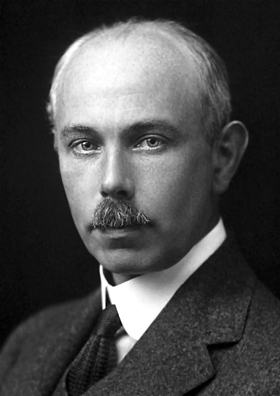
\includegraphics[width=\linewidth]{images/book3/aston.jpg}
\end{minipage}\hspace{0.02\linewidth}%
\begin{minipage}[t]{0.24\linewidth}
\vspace{0pt}
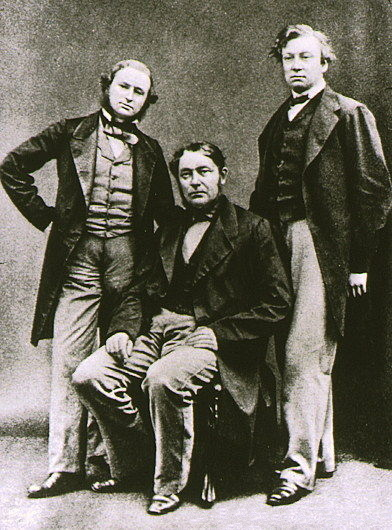
\includegraphics[width=\linewidth]{images/book3/kirchhoff-bunsen.jpg}
\end{minipage}\hfill
\begin{minipage}[t]{0.54\linewidth}
\vspace{0pt}
Gustav Kirchhoff dan Robert Bunsen menunjukkan sekitar tahun 1860 bahwa
setiap unsur memberikan garis-garisnya sendiri dalam nyala, dan menemukan
sesium dan rubidium melalui garis-garisnya yang belum dikenal.
Spektrograf massa Francis Aston, sejak 1919, menunjukkan bahwa sebagian
besar unsur adalah campuran isotop; ia menerima Hadiah Nobel Kimia 1922.
(Foto: Aston, pembuat tidak diketahui, domain publik; Kirchhoff, Bunsen,
dan Henry Roscoe pada tahun 1862, dari koleksi Roscoe, domain publik;
Wikimedia Commons.)
\end{minipage}
\end{history}

\section{Latihan}

\begin{exercise}[$\star$]\label{exo:b2:mass-spec-atomic:1}
Tentukan $m/z$ untuk: \omterm{def:b2:mass-spec-atomic:molecular-ion}{ion molekul} benzena \ce{C6H6}; ion bermassa
\qty{400}{u} yang membawa dua muatan; molekul kafeina yang terprotonasi
(\ce{C8H10N4O2}, massa nominal 194) yang terbentuk melalui semprot listrik.
\end{exercise}

\begin{exercise}[$\star$]\label{exo:b2:mass-spec-atomic:2}
Sebuah senyawa C, H, N, dan O mempunyai \omterm{def:b2:mass-spec-atomic:molecular-ion}{ion molekul} pada $m/z$ 73. Apa yang
dapat dikatakan tentang atom-atom nitrogennya? Usulkan sebuah rumus.
\end{exercise}

\begin{exercise}[$\star$]\label{exo:b2:mass-spec-atomic:3}
Sebuah kelompok \omterm{def:b2:mass-spec-atomic:molecular-ion}{ion molekul} memperlihatkan dua puncak yang berjarak dua
satuan, dengan tinggi yang hampir sama. Kelompok lain memperlihatkan dua
puncak yang berjarak dua satuan dengan rasio 3 : 1. Halogen manakah?
\end{exercise}

\begin{exercise}[$\star$]\label{exo:b2:mass-spec-atomic:4}
Sebuah garam mewarnai nyala menjadi kuning; garam lain merah tua.
Identifikasilah unsur-unsurnya dan tuliskan panjang gelombang
garis-garisnya.
\end{exercise}

\begin{exercise}[$\star\star$]\label{exo:b2:mass-spec-atomic:5}
Sebuah hidrokarbon mempunyai $M$ pada 100 \% dan $M+1$ pada 6.7 \%. Berapa atom karbon yang dikandungnya?
\end{exercise}

\begin{exercise}[$\star\star$]\label{exo:b2:mass-spec-atomic:6}
Hitunglah massa eksak \ce{CO}, \ce{N2}, dan \ce{C2H4} serta daya pisah yang
diperlukan untuk memisahkan setiap pasangan.
\end{exercise}

\begin{exercise}[$\star\star$]\label{exo:b2:mass-spec-atomic:7}
Spektrum EI pentan-3-on memperlihatkan puncak pada 86, 57 (\omterm{def:b2:mass-spec-atomic:spectrum}{puncak dasar}), dan 29. Tetapkan asal-usulnya.
\end{exercise}

\begin{exercise}[$\star\star$]\label{exo:b2:mass-spec-atomic:8}
Spektrum pentan-2-on memperlihatkan puncak pada 86, 71, 58, dan 43 (\omterm{def:b2:mass-spec-atomic:spectrum}{puncak
dasar}). Tetapkan asal-usulnya, dan jelaskan mengapa pentan-3-on hanya
memperlihatkan puncak kecil pada 58.
\end{exercise}

\begin{exercise}[$\star\star$]\label{exo:b2:mass-spec-atomic:9}
Standar tembaga pada 1.0, 2.0, 3.0, dan \qty{4.0}{mg/L} memberikan absorbans
0.052, 0.104, 0.155, dan 0.207; sebuah sampel memberikan 0.128 (data latihan).
Hitunglah konsentrasi tembaganya.
\end{exercise}

\begin{exercise}[$\star\star\star$]\label{exo:b2:mass-spec-atomic:10}
Dalam penganalisis waktu terbang, $L = \qty{1.00}{m}$ dan $U = \qty{20.0}{kV}$.
Hitunglah waktu terbang ion bermuatan tunggal bermassa \qty{1000}{u}, dan
selang waktu yang memisahkannya dari ion bermassa \qty{1001}{u}.
\end{exercise}

\begin{exercise}[$\star\star\star$]\label{exo:b2:mass-spec-atomic:11}
Hitunglah kelompok \omterm{def:b2:mass-spec-atomic:molecular-ion}{ion molekul} diklorometana, \ce{CH2Cl2}: nilai-nilai $m/z$
dan intensitas relatifnya.
\end{exercise}

\begin{exercise}[$\star\star\star$]\label{exo:b2:mass-spec-atomic:12}
Dalam ICP-MS, \ce{^{40}Ar^{16}O+} mengganggu \ce{^{56}Fe+}. Hitunglah daya
pisah yang diperlukan untuk memisahkan keduanya, dan usulkan jalan keluar
lain.
\end{exercise}

\section{Soal: Sebuah Halida yang Tidak Diketahui}

\begin{problem}[{Soal akhir pekan --- kelompok ion molekul dengan klor dan
brom, banyaknya karbon, fragmen-fragmen, dan sebuah struktur yang
diperiksa terhadap setiap puncak}]
\label{pb:b2:mass-spec-atomic:1}
Sebuah cairan tak berwarna, yang terelusi sebagai satu puncak dalam
\omterm{def:b2:chromatography:techniques}{kromatografi gas}, memberikan \omterm{def:b2:mass-spec-atomic:spectrum}{spektrum massa} EI di bawah ini (data NIST
WebBook). Puncak-puncak utama ($m/z$: intensitas relatif): 156: 14.5; 157: 0.5; 158: 18.6; 159: 0.6; 160:
4.4; 107: 6.7; 109: 6.3; 93: 3.3; 95: 2.9; 77: 59; 79: 18.7; 76: 39.5; 49: 12.9; 51: 4.3; 41: 100; 39:
26.2; 27: 24.6. Kelimpahan isotop: \ce{^{35}Cl} 0.758, \ce{^{37}Cl} 0.242, \ce{^{79}Br} 0.5069,
\ce{^{81}Br} 0.4931, \ce{^{12}C} 0.989, \ce{^{13}C} 0.011.
% ledger: ms:bromochloropropane, iso:Cl35, iso:Cl37, iso:Br79, iso:Br81, iso:C12, iso:C13, mass:C12, mass:H1, mass:Br79, mass:Cl35

\begin{center}
\begin{tikzpicture}
\begin{axis}[width=0.8\linewidth, height=4.6cm, xmin=20, xmax=170, ymin=0, ymax=112,
  xlabel={$m/z$}, ylabel={intensitas relatif}, label style={font=\small},
  tick label style={font=\scriptsize}, ycomb, xtick={27,41,49,77,93,107,122,156}]
\addplot[omDef, thick] table[x=mz, y=I] {figdata/out/bachelor-2-mass-spectra-d.dat};
\end{axis}
\end{tikzpicture}
\end{center}
% figdata: bachelor-2/mass-spectra.py part d

\medskip
\noindent\textbf{Bagian I --- \omterm{def:b2:mass-spec-atomic:molecular-ion}{Ion molekul}.}
\begin{enumerate}
  \item Puncak-puncak manakah yang membentuk kelompok \omterm{def:b2:mass-spec-atomic:molecular-ion}{ion molekul}? Mengapa
        kelompok itu bukan satu puncak saja?
  \item Halogen manakah yang diisyaratkan oleh kelompok tiga puncak yang berjarak 2?
  \item Berapa massa nominal bentuk isotopik yang paling ringan?
  \item Apa yang dikatakan oleh \omterm{def:b2:mass-spec-atomic:nitrogen-rule}{aturan nitrogen}?
  \item Kurangkan satu \ce{^{79}Br} dan satu \ce{^{35}Cl}: apa yang tersisa,
        dan fragmen hidrokarbon manakah yang bermassa itu?
  \item Usulkan rumus molekul dan tentukan derajat ketidakjenuhannya.
\end{enumerate}

\medskip
\noindent\textbf{Bagian II --- Karbon dan massa eksak.}
\begin{enumerate}[resume]
  \item Dari rasio 157/156, perkirakan banyaknya karbon.
  \item Mengapa perkiraan itu kasar di sini?
  \item Bentuk-bentuk isotopik manakah yang menyumbang puncak pada 158?
  \item Hitunglah \omterm{def:b2:mass-spec-atomic:exact-mass}{massa monoisotopik} \omterm{def:b2:mass-spec-atomic:molecular-ion}{ion molekul}.
  \item \ce{C10H20O} juga mempunyai massa nominal 156 (eksak 156.151). Daya
        pisah berapakah yang memisahkan keduanya?
  \item Apakah \omterm{def:b2:mass-spec-atomic:molecular-ion}{ion molekul} senyawa dengan ikatan C=C dan halogen yang sama
        akan mempunyai massa nominal yang berbeda?
\end{enumerate}

\medskip
\noindent\textbf{Bagian III --- Fragmen.}
\begin{enumerate}[resume]
  \item Pasangan 77/79 berasio 3 : 1. Atom manakah yang hilang, dan ion apakah itu?
  \item Jelaskan puncak pada 76.
  \item Tetapkan asal-usul \omterm{def:b2:mass-spec-atomic:spectrum}{puncak dasar} pada 41.
  \item Tetapkan asal-usul pasangan 49/51.
  \item Tetapkan asal-usul pasangan 93/95 dan 107/109.
  \item Mengapa atom brom lebih mudah lepas daripada atom klor?
  \item 1-Bromo-1-kloropropana akan memberikan \ce{CHBrCl+} pada 127, 129,
        dan 131. Apakah spektrum itu mendukungnya?
\end{enumerate}

\medskip
\noindent\textbf{Bagian IV --- Struktur.}
\begin{enumerate}[resume]
  \item Usulkan strukturnya.
  \item Periksalah bahwa struktur itu menjelaskan setiap puncak yang didaftar.
  \item Dapatkah terjadi \omterm{def:b2:mass-spec-atomic:fragmentation}{penataan ulang McLafferty}? Mengapa?
  \item Gambarlah isomer yang akan memberikan puncak kuat pada $m/z$ 63/65 dan tidak ada puncak pada 49/51.
  \item Bentuk-bentuk isotopik manakah yang membentuk puncak pada 160?
  \item Dari kelimpahan isotop, hitunglah rasio puncak $M$, $M+2$, dan $M+4$
        untuk satu klor dan satu brom, dan bandingkan dengan spektrumnya.
\end{enumerate}
\end{problem}
